%%%%%%%%%%%%%%%%%%%%%%%%%%%%%%%%%%%%%%%%%
% The Legrand Orange Book
% LaTeX Template
% Version 2.1.1 (14/2/16)
%
% This template has been downloaded from:
% http://www.LaTeXTemplates.com
%
% Original author:
% Mathias Legrand (legrand.mathias@gmail.com) with modifications by:
% Vel (vel@latextemplates.com)
%
% License:
% CC BY-NC-SA 3.0 (http://creativecommons.org/licenses/by-nc-sa/3.0/)
%
% Compiling this template:
% This template uses biber for its bibliography and makeindex for its index.
% When you first open the template, compile it from the command line with the 
% commands below to make sure your LaTeX distribution is configured correctly:
%
% 1) pdflatex main
% 2) makeindex main.idx -s StyleInd.ist
% 3) biber main
% 4) pdflatex main x 2
%
% After this, when you wish to update the bibliography/index use the appropriate
% command above and make sure to compile with pdflatex several times 
% afterwards to propagate your changes to the document.
%
% This template also uses a number of packages which may need to be
% updated to the newest versions for the template to compile. It is strongly
% recommended you update your LaTeX distribution if you have any
% compilation errors.
%
% Important note:
% Chapter heading images should have a 2:1 width:height ratio,
% e.g. 920px width and 460px height.
%
%%%%%%%%%%%%%%%%%%%%%%%%%%%%%%%%%%%%%%%%%

%----------------------------------------------------------------------------------------
%	PACKAGES AND OTHER DOCUMENT CONFIGURATIONS
%----------------------------------------------------------------------------------------

\documentclass[11pt,oneside,fleqn]{book} % Default font size and left-justified equations

%----------------------------------------------------------------------------------------

%%%%%%%%%%%%%%%%%%%%%%%%%%%%%%%%%%%%%%%%%
% The Legrand Orange Book
% Structural Definitions File
% Version 2.0 (9/2/15)
%
% Original author:
% Mathias Legrand (legrand.mathias@gmail.com) with modifications by:
% Vel (vel@latextemplates.com)
% 
% This file has been downloaded from:
% http://www.LaTeXTemplates.com
%
% License:
% CC BY-NC-SA 3.0 (http://creativecommons.org/licenses/by-nc-sa/3.0/)
%
%%%%%%%%%%%%%%%%%%%%%%%%%%%%%%%%%%%%%%%%%

%----------------------------------------------------------------------------------------
%	VARIOUS REQUIRED PACKAGES AND CONFIGURATIONS
%----------------------------------------------------------------------------------------

\usepackage[top=3cm,bottom=3cm,left=3cm,right=3cm,headsep=10pt,a4paper]{geometry} % Page margins

\usepackage{graphicx} % Required for including pictures
\graphicspath{{Pictures/}} % Specifies the directory where pictures are stored
\usepackage{gensymb}
\usepackage{lipsum} % Inserts dummy text

\usepackage{tikz} % Required for drawing custom shapes

\usepackage[english]{babel} % English language/hyphenation

\usepackage{enumitem} % Customize lists
\setlist{nolistsep} % Reduce spacing between bullet points and numbered lists

\usepackage{booktabs} % Required for nicer horizontal rules in tables

\usepackage{xcolor} % Required for specifying colors by name
\definecolor{ocre}{RGB}{100,100,100} % Define the orange color used for highlighting throughout the book

%----------------------------------------------------------------------------------------
%	FONTS
%----------------------------------------------------------------------------------------

\usepackage{avant} % Use the Avantgarde font for headings
%\usepackage{times} % Use the Times font for headings
\usepackage{mathptmx} % Use the Adobe Times Roman as the default text font together with math symbols from the Sym­bol, Chancery and Com­puter Modern fonts

\usepackage{microtype} % Slightly tweak font spacing for aesthetics
\usepackage[utf8]{inputenc} % Required for including letters with accents
\usepackage[T1]{fontenc} % Use 8-bit encoding that has 256 glyphs

%----------------------------------------------------------------------------------------
%	BIBLIOGRAPHY AND INDEX
%----------------------------------------------------------------------------------------

\usepackage{csquotes}
\usepackage[style=alphabetic,citestyle=numeric,sorting=nyt,sortcites=true,autopunct=true,autolang=hyphen,hyperref=true,abbreviate=false,backref=true,backend=biber,defernumbers=true]{biblatex}
\addbibresource{bibliography.bib} % BibTeX bibliography file
\defbibheading{bibempty}{}

\usepackage{calc} % For simpler calculation - used for spacing the index letter headings correctly
\usepackage{makeidx} % Required to make an index
\makeindex % Tells LaTeX to create the files required for indexing

%----------------------------------------------------------------------------------------
%	MAIN TABLE OF CONTENTS
%----------------------------------------------------------------------------------------

\usepackage{titletoc} % Required for manipulating the table of contents

\contentsmargin{0cm} % Removes the default margin

% Part text styling
\titlecontents{part}[0cm]
{\addvspace{20pt}\centering\large\bfseries}
{}
{}
{}

% Chapter text styling
\titlecontents{chapter}[1.25cm] % Indentation
{\addvspace{12pt}\large\sffamily\bfseries} % Spacing and font options for chapters
{\color{ocre!60}\contentslabel[\Large\thecontentslabel]{1.25cm}\color{ocre}} % Chapter number
{\color{ocre}}  
{\color{ocre!60}\normalsize\;\titlerule*[.5pc]{.}\;\thecontentspage} % Page number

% Section text styling
\titlecontents{section}[1.25cm] % Indentation
{\addvspace{3pt}\sffamily\bfseries} % Spacing and font options for sections
{\contentslabel[\thecontentslabel]{1.25cm}} % Section number
{}
{\hfill\color{black}\thecontentspage} % Page number
[]

% Subsection text styling
\titlecontents{subsection}[1.25cm] % Indentation
{\addvspace{1pt}\sffamily\small} % Spacing and font options for subsections
{\contentslabel[\thecontentslabel]{1.25cm}} % Subsection number
{}
{\ \titlerule*[.5pc]{.}\;\thecontentspage} % Page number
[]

% List of figures
\titlecontents{figure}[0em]
{\addvspace{-5pt}\sffamily}
{\thecontentslabel\hspace*{1em}}
{}
{\ \titlerule*[.5pc]{.}\;\thecontentspage}
[]

% List of tables
\titlecontents{table}[0em]
{\addvspace{-5pt}\sffamily}
{\thecontentslabel\hspace*{1em}}
{}
{\ \titlerule*[.5pc]{.}\;\thecontentspage}
[]

%----------------------------------------------------------------------------------------
%	MINI TABLE OF CONTENTS IN PART HEADS
%----------------------------------------------------------------------------------------

% Chapter text styling
\titlecontents{lchapter}[0em] % Indenting
{\addvspace{15pt}\large\sffamily\bfseries} % Spacing and font options for chapters
{\color{ocre}\contentslabel[\Large\thecontentslabel]{1.25cm}\color{ocre}} % Chapter number
{}  
{\color{ocre}\normalsize\sffamily\bfseries\;\titlerule*[.5pc]{.}\;\thecontentspage} % Page number

% Section text styling
\titlecontents{lsection}[0em] % Indenting
{\sffamily\small} % Spacing and font options for sections
{\contentslabel[\thecontentslabel]{1.25cm}} % Section number
{}
{}

% Subsection text styling
\titlecontents{lsubsection}[.5em] % Indentation
{\normalfont\footnotesize\sffamily} % Font settings
{}
{}
{}

%----------------------------------------------------------------------------------------
%	PAGE HEADERS
%----------------------------------------------------------------------------------------

\usepackage{fancyhdr} % Required for header and footer configuration

\pagestyle{fancy}
\renewcommand{\chaptermark}[1]{\markboth{\sffamily\normalsize\bfseries\chaptername\ \thechapter.\ #1}{}} % Chapter text font settings
\renewcommand{\sectionmark}[1]{\markright{\sffamily\normalsize\thesection\hspace{5pt}#1}{}} % Section text font settings
\fancyhf{} \fancyhead[LE,RO]{\sffamily\normalsize\thepage} % Font setting for the page number in the header
\fancyhead[LO]{\rightmark} % Print the nearest section name on the left side of odd pages
\fancyhead[RE]{\leftmark} % Print the current chapter name on the right side of even pages
\renewcommand{\headrulewidth}{0.5pt} % Width of the rule under the header
\addtolength{\headheight}{2.5pt} % Increase the spacing around the header slightly
\renewcommand{\footrulewidth}{0pt} % Removes the rule in the footer
\fancypagestyle{plain}{\fancyhead{}\renewcommand{\headrulewidth}{0pt}} % Style for when a plain pagestyle is specified

% Removes the header from odd empty pages at the end of chapters
% \makeatletter
% \renewcommand{\cleardoublepage}{
% \clearpage\ifodd\c@page\else
% \hbox{}
% \vspace*{\fill}
% \thispagestyle{empty}
% \newpage
% \fi}

%----------------------------------------------------------------------------------------
%	THEOREM STYLES
%----------------------------------------------------------------------------------------

\usepackage{amsmath,amsfonts,amssymb,amsthm} % For math equations, theorems, symbols, etc

\newcommand{\intoo}[2]{\mathopen{]}#1\,;#2\mathclose{[}}
\newcommand{\ud}{\mathop{\mathrm{{}d}}\mathopen{}}
\newcommand{\intff}[2]{\mathopen{[}#1\,;#2\mathclose{]}}
\newtheorem{notation}{Notation}[chapter]

% Boxed/framed environments
\newtheoremstyle{ocrenumbox}% % Theorem style name
{0pt}% Space above
{0pt}% Space below
{\normalfont}% % Body font
{}% Indent amount
{\small\bf\sffamily\color{ocre}}% % Theorem head font
{\;}% Punctuation after theorem head
{0.25em}% Space after theorem head
{\small\sffamily\color{ocre}\thmname{#1}\nobreakspace\thmnumber{\@ifnotempty{#1}{}\@upn{#2}}% Theorem text (e.g. Theorem 2.1)
\thmnote{\nobreakspace\the\thm@notefont\sffamily\bfseries\color{black}---\nobreakspace#3.}} % Optional theorem note
\renewcommand{\qedsymbol}{$\blacksquare$}% Optional qed square

\newtheoremstyle{blacknumex}% Theorem style name
{5pt}% Space above
{5pt}% Space below
{\normalfont}% Body font
{} % Indent amount
{\small\bf\sffamily}% Theorem head font
{\;}% Punctuation after theorem head
{0.25em}% Space after theorem head
{\small\sffamily{\tiny\ensuremath{\blacksquare}}\nobreakspace\thmname{#1}\nobreakspace\thmnumber{\@ifnotempty{#1}{}\@upn{#2}}% Theorem text (e.g. Theorem 2.1)
\thmnote{\nobreakspace\the\thm@notefont\sffamily\bfseries---\nobreakspace#3.}}% Optional theorem note

\newtheoremstyle{blacknumbox} % Theorem style name
{0pt}% Space above
{0pt}% Space below
{\normalfont}% Body font
{}% Indent amount
{\small\bf\sffamily}% Theorem head font
{\;}% Punctuation after theorem head
{0.25em}% Space after theorem head
{\small\sffamily\thmname{#1}\nobreakspace\thmnumber{\@ifnotempty{#1}{}\@upn{#2}}% Theorem text (e.g. Theorem 2.1)
\thmnote{\nobreakspace\the\thm@notefont\sffamily\bfseries---\nobreakspace#3.}}% Optional theorem note

% Non-boxed/non-framed environments
\newtheoremstyle{ocrenum}% % Theorem style name
{5pt}% Space above
{5pt}% Space below
{\normalfont}% % Body font
{}% Indent amount
{\small\bf\sffamily\color{ocre}}% % Theorem head font
{\;}% Punctuation after theorem head
{0.25em}% Space after theorem head
{\small\sffamily\color{ocre}\thmname{#1}\nobreakspace\thmnumber{\@ifnotempty{#1}{}\@upn{#2}}% Theorem text (e.g. Theorem 2.1)
\thmnote{\nobreakspace\the\thm@notefont\sffamily\bfseries\color{black}---\nobreakspace#3.}} % Optional theorem note
\renewcommand{\qedsymbol}{$\blacksquare$}% Optional qed square
\makeatother

% Defines the theorem text style for each type of theorem to one of the three styles above
\newcounter{dummy} 
\numberwithin{dummy}{section}
\theoremstyle{ocrenumbox}
\newtheorem{theoremeT}[dummy]{Theorem}
\newtheorem{problem}{Problem}[chapter]
\newtheorem{exerciseT}{Exercise}[chapter]
\theoremstyle{blacknumex}
\newtheorem{exampleT}{Example}[chapter]
\theoremstyle{blacknumbox}
\newtheorem{vocabulary}{Vocabulary}[chapter]
\newtheorem{definitionT}{Definition}[section]
\newtheorem{corollaryT}[dummy]{Corollary}
\theoremstyle{ocrenum}
\newtheorem{proposition}[dummy]{Proposition}

%----------------------------------------------------------------------------------------
%	DEFINITION OF COLORED BOXES
%----------------------------------------------------------------------------------------

\RequirePackage[framemethod=default]{mdframed} % Required for creating the theorem, definition, exercise and corollary boxes

% Theorem box
\newmdenv[skipabove=7pt,
skipbelow=7pt,
backgroundcolor=black!5,
linecolor=ocre,
innerleftmargin=5pt,
innerrightmargin=5pt,
innertopmargin=5pt,
leftmargin=0cm,
rightmargin=0cm,
innerbottommargin=5pt]{tBox}

% Exercise box	  
\newmdenv[skipabove=7pt,
skipbelow=7pt,
rightline=false,
leftline=true,
topline=false,
bottomline=false,
backgroundcolor=ocre!10,
linecolor=ocre,
innerleftmargin=5pt,
innerrightmargin=5pt,
innertopmargin=5pt,
innerbottommargin=5pt,
leftmargin=0cm,
rightmargin=0cm,
linewidth=4pt]{eBox}	

% Definition box
\newmdenv[skipabove=7pt,
skipbelow=7pt,
rightline=false,
leftline=true,
topline=false,
bottomline=false,
linecolor=ocre,
innerleftmargin=5pt,
innerrightmargin=5pt,
innertopmargin=0pt,
leftmargin=0cm,
rightmargin=0cm,
linewidth=4pt,
innerbottommargin=0pt]{dBox}	

% Corollary box
\newmdenv[skipabove=7pt,
skipbelow=7pt,
rightline=false,
leftline=true,
topline=false,
bottomline=false,
linecolor=gray,
backgroundcolor=black!5,
innerleftmargin=5pt,
innerrightmargin=5pt,
innertopmargin=5pt,
leftmargin=0cm,
rightmargin=0cm,
linewidth=4pt,
innerbottommargin=5pt]{cBox}

% Creates an environment for each type of theorem and assigns it a theorem text style from the "Theorem Styles" section above and a colored box from above
\newenvironment{theorem}{\begin{tBox}\begin{theoremeT}}{\end{theoremeT}\end{tBox}}
\newenvironment{exercise}{\begin{eBox}\begin{exerciseT}}{\hfill{\color{ocre}\tiny\ensuremath{\blacksquare}}\end{exerciseT}\end{eBox}}				  
\newenvironment{definition}{\begin{dBox}\begin{definitionT}}{\end{definitionT}\end{dBox}}	
\newenvironment{example}{\begin{exampleT}}{\hfill{\tiny\ensuremath{\blacksquare}}\end{exampleT}}		
\newenvironment{corollary}{\begin{cBox}\begin{corollaryT}}{\end{corollaryT}\end{cBox}}	

%----------------------------------------------------------------------------------------
%	REMARK ENVIRONMENT
%----------------------------------------------------------------------------------------

\newenvironment{remark}{\par\vspace{10pt}\small % Vertical white space above the remark and smaller font size
\begin{list}{}{
\leftmargin=35pt % Indentation on the left
\rightmargin=25pt}\item\ignorespaces % Indentation on the right
\makebox[-2.5pt]{\begin{tikzpicture}[overlay]
\node[draw=ocre!60,line width=1pt,circle,fill=ocre!25,font=\sffamily\bfseries,inner sep=2pt,outer sep=0pt] at (-15pt,0pt){\textcolor{ocre}{R}};\end{tikzpicture}} % Orange R in a circle
\advance\baselineskip -1pt}{\end{list}\vskip5pt} % Tighter line spacing and white space after remark

%----------------------------------------------------------------------------------------
%	SECTION NUMBERING IN THE MARGIN
%----------------------------------------------------------------------------------------

\makeatletter
\renewcommand{\@seccntformat}[1]{\llap{\textcolor{ocre}{\csname the#1\endcsname}\hspace{1em}}}                    
\renewcommand{\section}{\@startsection{section}{1}{\z@}
{-4ex \@plus -1ex \@minus -.4ex}
{1ex \@plus.2ex }
{\normalfont\large\sffamily\bfseries}}
\renewcommand{\subsection}{\@startsection {subsection}{2}{\z@}
{-3ex \@plus -0.1ex \@minus -.4ex}
{0.5ex \@plus.2ex }
{\normalfont\sffamily\bfseries}}
\renewcommand{\subsubsection}{\@startsection {subsubsection}{3}{\z@}
{-2ex \@plus -0.1ex \@minus -.2ex}
{.2ex \@plus.2ex }
{\normalfont\small\sffamily\bfseries}}                        
\renewcommand\paragraph{\@startsection{paragraph}{4}{\z@}
{-2ex \@plus-.2ex \@minus .2ex}
{.1ex}
{\normalfont\small\sffamily\bfseries}}

%----------------------------------------------------------------------------------------
%	PART HEADINGS
%----------------------------------------------------------------------------------------

% numbered part in the table of contents
\newcommand{\@mypartnumtocformat}[2]{%
\setlength\fboxsep{0pt}%
\noindent\colorbox{ocre!20}{\strut\parbox[c][.7cm]{\ecart}{\color{ocre!70}\Large\sffamily\bfseries\centering#1}}\hskip\esp\colorbox{ocre!40}{\strut\parbox[c][.7cm]{\linewidth-\ecart-\esp}{\Large\sffamily\centering#2}}}%
%%%%%%%%%%%%%%%%%%%%%%%%%%%%%%%%%%
% unnumbered part in the table of contents
\newcommand{\@myparttocformat}[1]{%
\setlength\fboxsep{0pt}%
\noindent\colorbox{ocre!40}{\strut\parbox[c][.7cm]{\linewidth}{\Large\sffamily\centering#1}}}%
%%%%%%%%%%%%%%%%%%%%%%%%%%%%%%%%%%
\newlength\esp
\setlength\esp{4pt}
\newlength\ecart
\setlength\ecart{1.2cm-\esp}
\newcommand{\thepartimage}{}%
\newcommand{\partimage}[1]{\renewcommand{\thepartimage}{#1}}%
\def\@part[#1]#2{%
\ifnum \c@secnumdepth >-2\relax%
\refstepcounter{part}%
\addcontentsline{toc}{part}{\texorpdfstring{\protect\@mypartnumtocformat{\thepart}{#1}}{\partname~\thepart\ ---\ #1}}
\else%
\addcontentsline{toc}{part}{\texorpdfstring{\protect\@myparttocformat{#1}}{#1}}%
\fi%
\startcontents%
\markboth{}{}%
{\thispagestyle{empty}%
\begin{tikzpicture}[remember picture,overlay]%
\node at (current page.north west){\begin{tikzpicture}[remember picture,overlay]%	
\fill[ocre!20](0cm,0cm) rectangle (\paperwidth,-\paperheight);
\node[anchor=north] at (4cm,-3.25cm){\color{ocre!40}\fontsize{220}{100}\sffamily\bfseries\@Roman\c@part}; 
\node[anchor=south east] at (\paperwidth-1cm,-\paperheight+1cm){\parbox[t][][t]{8.5cm}{
\printcontents{l}{0}{\setcounter{tocdepth}{1}}%
}};
\node[anchor=north east] at (\paperwidth-1.5cm,-3.25cm){\parbox[t][][t]{15cm}{\strut\raggedleft\color{white}\fontsize{30}{30}\sffamily\bfseries#2}};
\end{tikzpicture}};
\end{tikzpicture}}%
\@endpart}
\def\@spart#1{%
\startcontents%
\phantomsection
{\thispagestyle{empty}%
\begin{tikzpicture}[remember picture,overlay]%
\node at (current page.north west){\begin{tikzpicture}[remember picture,overlay]%	
\fill[ocre!20](0cm,0cm) rectangle (\paperwidth,-\paperheight);
\node[anchor=north east] at (\paperwidth-1.5cm,-3.25cm){\parbox[t][][t]{15cm}{\strut\raggedleft\color{white}\fontsize{30}{30}\sffamily\bfseries#1}};
\end{tikzpicture}};
\end{tikzpicture}}
\addcontentsline{toc}{part}{\texorpdfstring{%
\setlength\fboxsep{0pt}%
\noindent\protect\colorbox{ocre!40}{\strut\protect\parbox[c][.7cm]{\linewidth}{\Large\sffamily\protect\centering #1\quad\mbox{}}}}{#1}}%
\@endpart}
% \def\@endpart{\vfil\newpage
% \if@twoside
% \if@openright
% \null
% \thispagestyle{empty}%
% \newpage
% \fi
% \fi
% \if@tempswa
% \twocolumn
% \fi}

%----------------------------------------------------------------------------------------
%	CHAPTER HEADINGS
%----------------------------------------------------------------------------------------

% A switch to conditionally include a picture, implemented by  Christian Hupfer
\newif\ifusechapterimage
\usechapterimagetrue
\newcommand{\thechapterimage}{}%
\newcommand{\chapterimage}[1]{\ifusechapterimage\renewcommand{\thechapterimage}{#1}\fi}%
\def\@makechapterhead#1{%
{\parindent \z@ \raggedright \normalfont
\ifnum \c@secnumdepth >\m@ne
\if@mainmatter
\begin{tikzpicture}[remember picture,overlay]
\node at (current page.north west)
{\begin{tikzpicture}[remember picture,overlay]
\node[anchor=north west,inner sep=0pt] at (0,0) {\ifusechapterimage\includegraphics[width=\paperwidth]{\thechapterimage}\fi};
\draw[anchor=west] (\Gm@lmargin,-9cm) node [line width=2pt,rounded corners=15pt,draw=ocre,fill=white,fill opacity=0.5,inner sep=15pt]{\strut\makebox[22cm]{}};
\draw[anchor=west] (\Gm@lmargin+.3cm,-9cm) node {\huge\sffamily\bfseries\color{black}\thechapter. #1\strut};
\end{tikzpicture}};
\end{tikzpicture}
\else
\begin{tikzpicture}[remember picture,overlay]
\node at (current page.north west)
{\begin{tikzpicture}[remember picture,overlay]
\node[anchor=north west,inner sep=0pt] at (0,0) {\ifusechapterimage\includegraphics[width=\paperwidth]{\thechapterimage}\fi};
\draw[anchor=west] (\Gm@lmargin,-9cm) node [line width=2pt,rounded corners=15pt,draw=ocre,fill=white,fill opacity=0.5,inner sep=15pt]{\strut\makebox[22cm]{}};
\draw[anchor=west] (\Gm@lmargin+.3cm,-9cm) node {\huge\sffamily\bfseries\color{black}#1\strut};
\end{tikzpicture}};
\end{tikzpicture}
\fi\fi\par\vspace*{270\p@}}}

%-------------------------------------------

\def\@makeschapterhead#1{%
\begin{tikzpicture}[remember picture,overlay]
\node at (current page.north west)
{\begin{tikzpicture}[remember picture,overlay]
\node[anchor=north west,inner sep=0pt] at (0,0) {\ifusechapterimage\includegraphics[width=\paperwidth]{\thechapterimage}\fi};
\draw[anchor=west] (\Gm@lmargin,-9cm) node [line width=2pt,rounded corners=15pt,draw=ocre,fill=white,fill opacity=0.5,inner sep=15pt]{\strut\makebox[22cm]{}};
\draw[anchor=west] (\Gm@lmargin+.3cm,-9cm) node {\huge\sffamily\bfseries\color{black}#1\strut};
\end{tikzpicture}};
\end{tikzpicture}
\par\vspace*{270\p@}}
\makeatother

%----------------------------------------------------------------------------------------
%	HYPERLINKS IN THE DOCUMENTS
%----------------------------------------------------------------------------------------

\usepackage{hyperref}
\hypersetup{hidelinks,colorlinks=false,breaklinks=true,urlcolor= ocre,bookmarksopen=false,pdftitle={Title},pdfauthor={Author}}
\usepackage{bookmark}
\bookmarksetup{
open,
numbered,
addtohook={%
\ifnum\bookmarkget{level}=0 % chapter
\bookmarksetup{bold}%
\fi
\ifnum\bookmarkget{level}=-1 % part
\bookmarksetup{color=ocre,bold}%
\fi
}
}
 % Insert the commands.tex file which contains the majority of the structure behind the template

\begin{document}

%----------------------------------------------------------------------------------------
%	TITLE PAGE
%----------------------------------------------------------------------------------------

\begingroup
\thispagestyle{empty}
\begin{tikzpicture}[remember picture,overlay]
\coordinate [below=13cm] (midpoint) at (current page.north);
\node at (current page.north west)
{\begin{tikzpicture}[remember picture,overlay]
\node[anchor=north west,inner sep=0pt] at (0,0) {
\includegraphics[width=\paperwidth]{background}}; % Background image
\draw[anchor=north] (midpoint) node [fill=ocre!30!white,fill opacity=0.6,text opacity=0.7,inner sep=0.3cm]{\Huge\centering\sffamily\parbox[c][][t]{\paperwidth}{\centering \textbf{USB 3.0 Plugin Module}\\[10pt] % Book title
{\huge Apurva Nandan}\\ % Subtitle
{\Large Supervised by Herbert P\"otzl} \\
{\Large Google Summer of Code '19}}}; % Author name
\end{tikzpicture}};
\end{tikzpicture}
\vfill
\endgroup
%----------------------------------------------------------------------------------------
%	COPYRIGHT PAGE
%----------------------------------------------------------------------------------------

\newpage
~\vfill
\thispagestyle{empty}

\noindent Copyright \copyright\ 2019 Apurva Nandan.\\ % Copyright notice

\noindent \textsc{apertus.org}\\ % URL

\noindent Licensed under the Creative Commons Attribution-NonCommercial 3.0 Unported License (the ``License''). You may not use this file except in compliance with the License. You may obtain a copy of the License at \url{http://creativecommons.org/licenses/by-nc/3.0}. Unless required by applicable law or agreed to in writing, software distributed under the License is distributed on an \textsc{``as is'' basis, without warranties or conditions of any kind}, either express or implied. See the License for the specific language governing permissions and limitations under the License.\\ % License information

\noindent \textit{First edition, August 2019} % Printing/edition date

%----------------------------------------------------------------------------------------
%	TABLE OF CONTENTS
%----------------------------------------------------------------------------------------

%\usechapterimagefalse % If you don't want to include a chapter image, use this to toggle images off - it can be enabled later with \usechapterimagetrue

\chapterimage{axiom_beta.png} % Table of contents heading image

\pagestyle{empty} % No headers

\tableofcontents % Print the table of contents itself

\cleardoublepage % Forces the first chapter to start on an odd page so it's on the right

\pagestyle{fancy} % Print headers again

%----------------------------------------------------------------------------------------
%	PART
%----------------------------------------------------------------------------------------

\part{Part One}
%----------------------------------------------------------------------------------------
%	CHAPTER 1
%----------------------------------------------------------------------------------------

\chapterimage{gsoc.jpg} % Chapter heading image

\chapter{GSoC'19 Project Report}

\section{Overview}\index{Overview}

The AXIOM Beta features PCIe x1 slots on the main board to allow optional plugin modules to extend the IO capabilities of the camera. One such module, the USB 3.0 plugin module, is designed by apertus$\degree$ Association to allow live stream of 4K video at 20+ FPS to a PC for video processing \& recording purposes. My aim in this GSoC project was to develop gearwork HDLs for the USB 3.0 Plugin Module that can provide a throughput of at least 3.0 Gbps from the AXIOM Beta camera to the PC with Bit Error Rate (BER) lower than $10^{-12}$.
\\


All the source code written by me during the period of GSoC'19 can be found here: 


\textcolor{blue}{\url{https://github.com/apurvanandan1997/usb_plug_mod_ber} }
\\
For detailed documentation of the gearwork of the USB 3.0 Plugin Module, please go to Part Two of this report 
%------------------------------------------------

\section{Community Bonding Period}\index{Community Bonding Period}
\begin{itemize}
  \item This period was mainly spent in setting up the work environment, both in terms of hardware \& software. Significant time was spent in getting acquainted with the existing code base of AXIOM Beta firmware and going through all the documentation relevant to the project.
  \item On the hardware side, I learnt how to operate the Remote Beta Camera available at Apertus$\degree$ Remote Testing Lab, Vienna. I also set up the USB 3.0 Plugin Module delivered by apertus$\degree$ locally with a XUPV5-LX110T FPGA. The local set up comprised of USB 3.0 Plugin Module attached to a breakout board powered by LDO regulator and connected to Virtex-5 using 6 LVDS connection pairs made using dupont cables.
  \item On the software side, all the manufacturer's tool, namely Xilinx Vivado, Xilinx ISE, Lattice Diamond and Modelsim, were installed on Ubuntu Linux, thereby allowing easy exchange of project source files with the mentors. Also, urJTAG 2018.9 was installed, which allowed programming the USB 3.0 Plugin module using Digilent XUP-USB-JTAG cable, to facilitate testing on the local hardware.

\end{itemize}



%------------------------------------------------

\section{First Coding Period}\index{First Coding Period}
\begin{itemize}
\item In this period, my major focus was on developing a FTDI FT601 controller for the plugin module that can receive 32-bit words at 100 MHz and transmit them to the D3XX driver running on a PC through USB 3.0 port, thereby providing 3.2 Gbps throughput.
\item The FT601 controller developed by me finally was able to provide a maximum throughput of 3.0 Gbps (limit of the FT601 chip  as per mentioned in it documentation). The catch here was that though the clock from FT601 is at 100 MHz but the internal FIFOs of this chip soon get full and the FIFO\_FULL output signal from the chip is asserted. This implies we get frequent pauses in data transfer of roughly 0.2us at about every 3ms which reduces average throughput from 3.2 Gbps down to 3.0 Gbps. In the case of the internal FIFO of the FT601 chip getting full, we need to stop sending data to the chip or else our gearwork's FIFO gets full and there is significant loss of data due to overflow. I wasn't able to resolve this in my project as the current technique of data transfer between the FPGAs is purely unidirectional and only some kind of feedback to the Transmitting FPGA (Zynq) from the Receiver FPGA (MachXO2) can resolve the issue. 
\item However, the fraction of time the internal FIFOs of the FT601 chip remains full is largely dependent on the CPU core resources and also on the efficiency of D3XX driver code. Using a light D3XX code with a powerful CPU setup, I was able to reach 3.0 Gbps with significantly less errors, although pausing the data input to the gearwork's FIFOs was able to provide 100\% accurate data throughput.
\item All tests were made on local and remote hardware. Code written by me in this period can be found here:\\ \textcolor{blue}{\url{https://github.com/apurvanandan1997/usb_plug_mod_ber/blob/master/MachXO2/src/ft601.vhd}}
\end{itemize}

\section{Second Coding Period}\index{Second Coding Period}

\begin{itemize}
\item In the second coding period, I implemented the HDLs for Transmitter/ MicroZed side of gearwork for Zynq XC7020 and Virtex-5 LX110T FPGAs. These HDLs comprised of the OSERDES blocks, 8b10b encoder (8b10b encoder and decoder were taken from \textcolor{blue}{\href{https://opencores.org/projects/8b10b_encdec}{OpenCores.org}} under GPLv3) and Fibonacci Pseudo-Random Number Generator for testing the BER of the LVDS connections.
\item The transmitter HDLs have been completed, yet there are additional features that can be incorporated in them, namely error reduction techniques like ECC CRC and use of more control symbols available for extending out of the band communication.
\item All transmitter HDLs written by me can be found in these two folders:\\
\textcolor{blue}{\url{https://github.com/apurvanandan1997/usb_plug_mod_ber/tree/master/Zynq}} \\
\textcolor{blue}{\url{https://github.com/apurvanandan1997/usb_plug_mod_ber/tree/master/Virtex-5}}
\end{itemize}

\section{Third Coding Period}\index{Third Coding Period}
\begin{itemize}
\item During the third coding period, I implemented most challenging part of this gearwork which were the HDLs for the receiver FPGA (MachXO2). These HDLs comprised of DDR x4 input gearing, link training, channel bonding of 5 LVDS lanes, 8:10 gearing, 8b10b decoder(8b10b encoder and decoder were taken from \textcolor{blue}{\href{https://opencores.org/projects/8b10b_encdec}{OpenCores.org}} under GPLv3), Clock Domain Crossing (CDC) FIFO and BER calculator.
\item After completing all these HDLs, I was able to run various important tests and measurements on USB 3.0 Plugin Module, among which the most significant was the BER testing of the LVDS lanes. The LVDS connection and the DDR x4 gearing primitive have been tested and verified using the BER testing model made by me. I hereby report the Bit Error Rate (BER) measured by my code on both local Virtex-5 hardware and remote AXIOM Beta hardware: \\
\textbf{BER measured on AXIOM Beta over 5 LVDS lanes at 375 MHz DDR ${\approx10^{-13}}$ \\
BER measured by Virtex-5 FPGA over 5 LVDS lanes at 375 MHz DDR ${\approx10^{-9}}$}
\\
\begin{table}[h!]
\centering
\begin{tabular}{l l l}
\toprule
\textbf{DDR Frequency (MHz)} & \textbf{Number of Bits Transferred} & \textbf{Number of Bit Errors}\\
\midrule
375.0 & $3.6\times10^{12}$ & 0 \\
350.0 & $4.3\times10^{10}$ & 0 \\
325.0 & $4.3\times10^{10}$ & 0 \\
300.0 & $4.3\times10^{10}$ & 0 \\
\bottomrule
\end{tabular}
\caption{BER results on Remote AXIOM Beta}
\end{table}
\\
\qquad
 Static delay have been used on the LVDS data lanes for aligning the edge of data transition with the high speed DDR clock edge. These static delays have been adjusted to work perfectly on the AXIOM Beta camera.
\item Due to courtesy of apertus$\degree$ Association, I was provided with the access to a remote AXIOM Beta setup at Remote Testing Lab, Vienna. I did all my final tests, which required greater degree of precision, on the remote hardware. This benefited us as the work of porting the code from my local hardware to AXIOM Beta was done along with in GSoC period only.  
\begin{figure}[h!]
\centering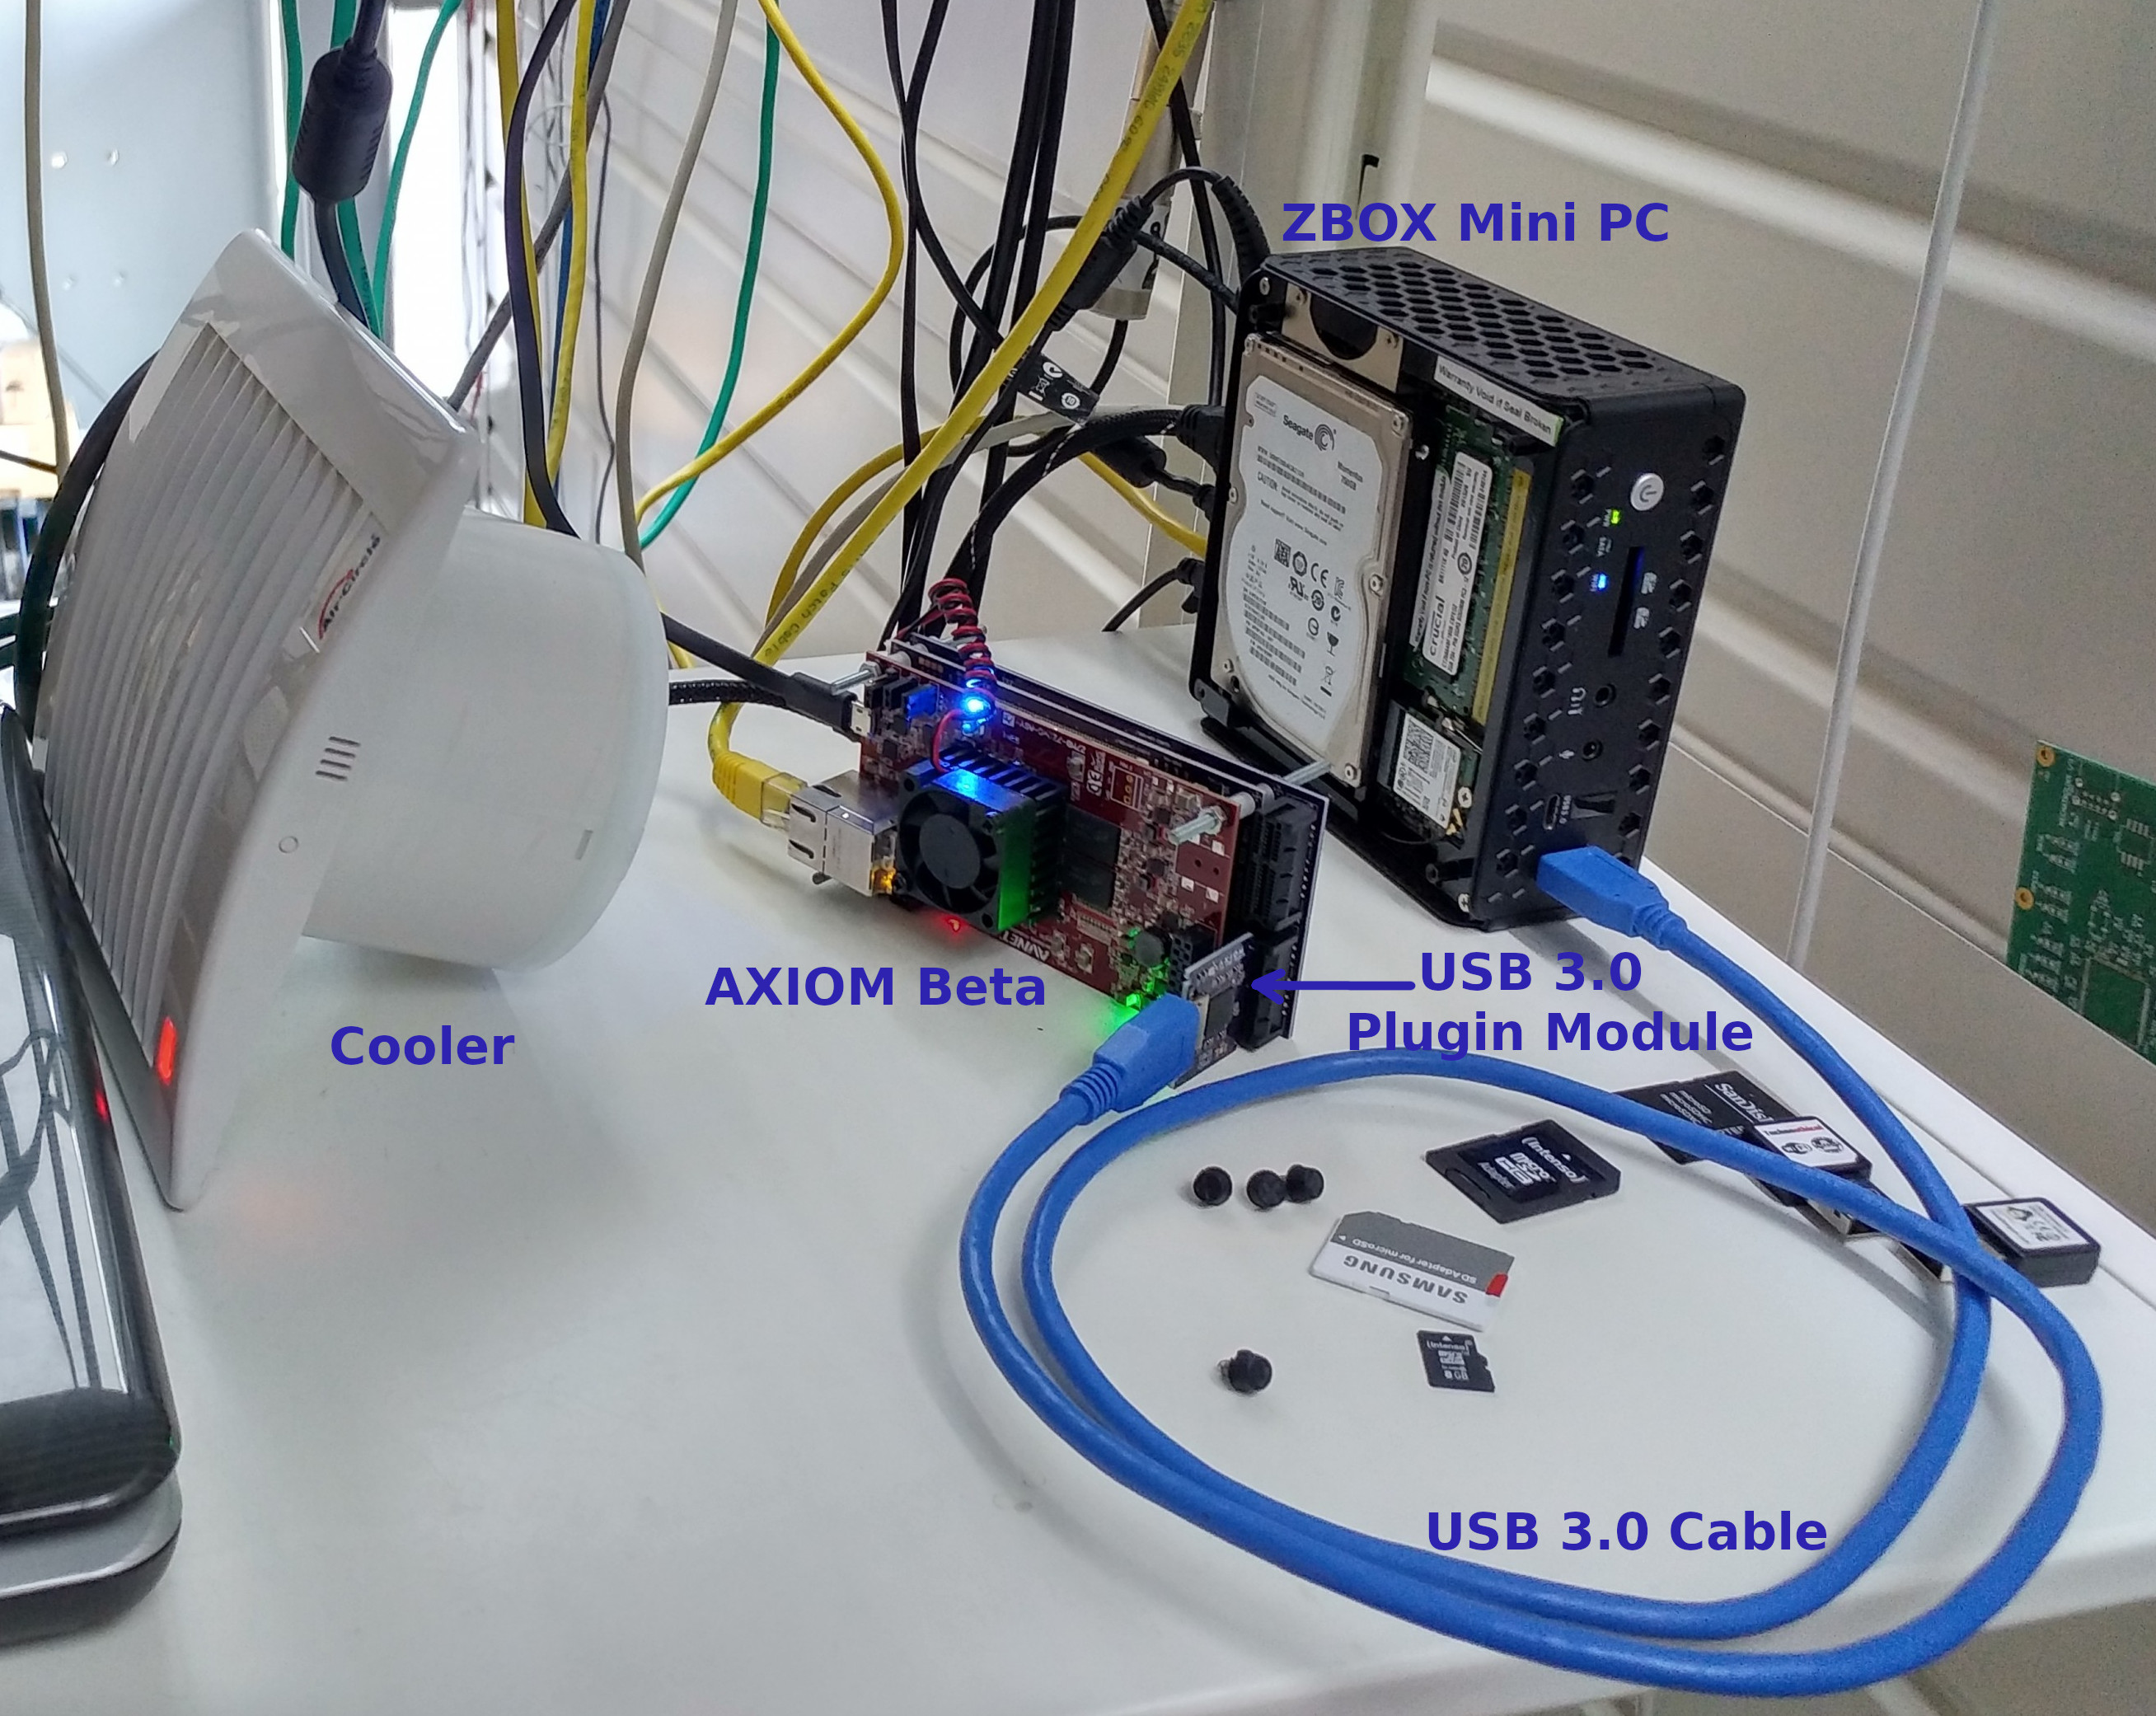
\includegraphics[scale=0.2]{remote_hardware.jpg}
\caption{Remote Hardware Setup (Photo credits: Sebastian Pichelhofer)}
\end{figure}
\item Locally, I had setup  following hardware for testing of BER of the plugin module. The local hardware smoothened the testing procedure and provided plenty of debugging options. In brief, this hardware comprised of similar setup as in AXIOM Beta, but instead of MicroZED board I used a Virtex-5 FPGA as a transmitter. The USB 3.0 Plugin module fits in a breakout board and thereby getting power from the LDO power supply, making the six LVDS connection from the Virtex-5 board, and getting programmed by the Xilinx Platform Cable DLC9LP. For programming the plugin module, a open source JTAG program named urJTAG was used, which was easily able to program the module within 1 second. The gearwork on receiver side remained identical with both the remote and local hardwares. 
\begin{figure}[h!]
\centering\includegraphics[scale=0.1]{Local_Hardware.png}
\caption{Local Hardware Setup}
\end{figure}

\item All receiver HDLs written by me, for the MachXO2 on the USB 3.0 plugin module, can be found on the following link:\\
\textcolor{blue}{\url{https://github.com/apurvanandan1997/usb_plug_mod_ber/tree/master/MachXO2}} \\
\end{itemize}

\section{Tasks Pending}\index{Tasks Pending}
\begin{itemize}
\item Implementing 40-bit to 32-bit gearing between the 5 8-bit LVDS lanes and the 32-bit CDC FT601 FIFO to allow data transfer along with the 32-bit BER. 
\item Incorporating feedback signals from the MachXO2 FPGA on USB 3.0 Plugin Module to the Zynq FPGA on the AXIOM Beta which would control the throughput of the data over the 5 LVDS lanes. 
\end{itemize}
%----------------------------------------------------------------------------------------
%	CHAPTER 2
%----------------------------------------------------------------------------------------
\chapterimage{opensource.png}
\chapter{Future Goals}
% \section{Error Correction Techniques}\index{Error Correction Techniques}
\section{Error Correction Techniques}\index{Error Correction Techniques}
Although the Bit Error Rate (BER) achieved over the 5 LVDS lanes on the AXIOM Beta is very low ( ${\approx10^{-12}}$), yet implementing the widely used error correction techniques like Error Correction Codes (ECC) \& Cyclic Redundancy Check (CRC) and can even allow us to overclock the DDR x4 primitives a little, thereby increasing the throughput through the LVDS lanes. 
\section{Featuring the FT602}\index{Featuring the FT602}
FTDI FT602 is a proprietary solution for plug and play type USB devices, so it doesn’t require any special software/drivers on most computers and is supported by many third party applications. FT602 takes the data input in form of 32-bit video data in YUV422 format at 100 MHz clock and also provides the option of compressed video data streaming. Hardware for USB 3.0 Plugin Module featuring the FT602 has recently been designed by apertus$\degree$ Association and is ready to allow furhter gearwork development. 
\section {Higher FPS at Same Throughput}\index{Higher FPS at Same Throughput} 
A 4K 12-bit video at 20+ FPS is definitely not sufficient as the CMV12000 sensor sends 4096x3072 sensel at up to 150 FPS. In GSoC'19, a Lossless JPEG 1992 Encoder on AXIOM Beta has been implemented by one of the students under apertus$\degree$ Association. To get higher frame rates, I would like to integrate my current gearwork with the JPEG encoder core thereby allowing video streaming at even higher FPS at same throughput by the USB 3.0 Plugin Module.
\section{Bidirectional Data Transfers}\index{Bidirectional Data Transfers}
As both FT601Q and FT602 allow bidirectional data transfer over USB 3.0, additional functionality and accessibility can be added to the USB 3.0 plugin module by making the data link from AXIOM Beta to the PC bidirectional by reverse implementation of the current gearwork. 
%----------------------------------------------------------------------------------------
%	PART
%----------------------------------------------------------------------------------------

\part{Part Two}

%----------------------------------------------------------------------------------------
%	CHAPTER 3
%----------------------------------------------------------------------------------------

\chapterimage{usb_plugin_mod.png} % Chapter heading image

\chapter{Gearwork Documentation}
\section{Overview}\index{Overview}
The RAW data captured from the CMV12000 sensor on the AXIOM Beta camera gets directly buffered on the DDR3 SDRAM of the MicroZED board. The main board of AXIOM Beta featrues PCIe x1 connectors which exposes 6 LVDS pairs (routed to the MicroZED board through JX connectors) and 8 GPIO pins (routed to West Routing Fabric (RFW)). In order to transmit the RAW video data from the DDR3 SDRAM of the AXIOM Beta, the USB 3.0 Plugin Module has been developed which would act as a 6-Lane LVDS connection to USB bridge between the camera and the PC. The USB 3.0 Plugin Module features a Lattice MachXO2 FPGA, on which the receiver gearwork logic has been implemented. A proprietary FTDI FT601 chip has been featured on this plugin module which inputs the a 32-bit data at 100 MHz through FIFOs and forwards them to  the USB 3.0 port, offloading the conversion of data packets to USB 3.0 protocol from the MachXO2 FPGA
\\ \\ 
The complete data flow from the DDR3 SDRAM on AXIOM Beta to the software driver on the connected PC can be described as follows:

\begin{figure}[h!]
\centering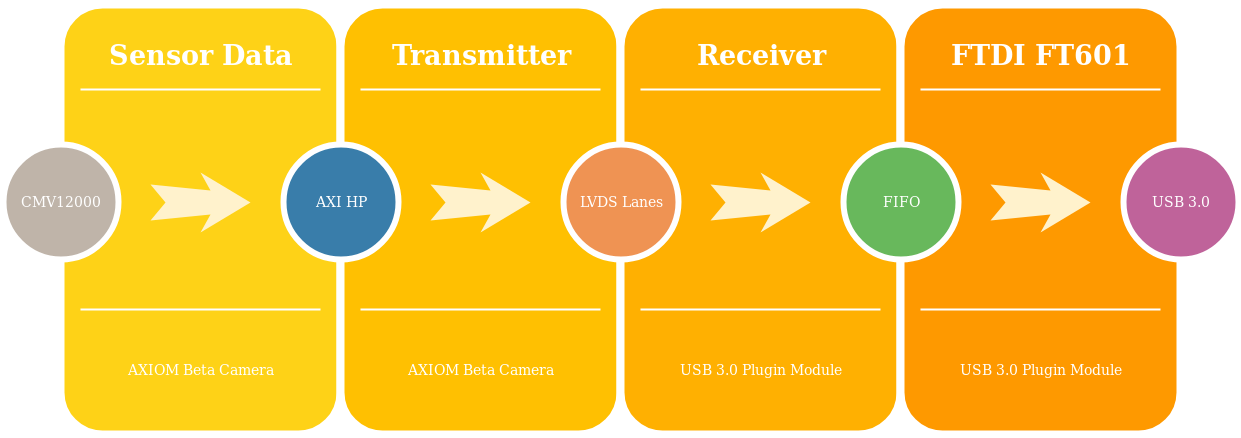
\includegraphics[scale=0.3]{dataflow.png}
\caption{Gearwork Overview}
\end{figure}

\section{Transmitter Gearwork}\index{Transmitter Gearwork}
\begin{figure}[h!]
\centering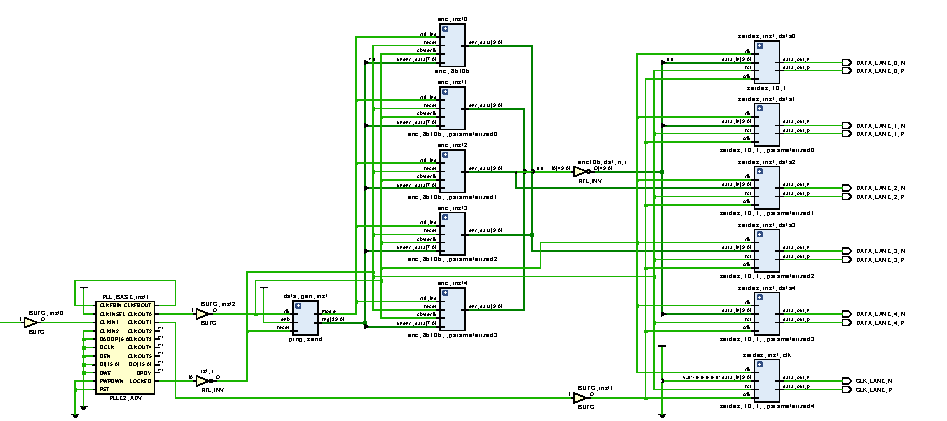
\includegraphics[scale=1]{Zynq_Schematic.pdf}
\caption{Zynq Gearwork Schematic}
\end{figure}
The above figure describes the transmitter part of model developed for BER testing.
\begin{itemize}
    \item The PLL\_ADV instance does the task of generating  the required clocks from the 50 MHz clock being received from the Zynq PS. The sclk is the fast serial clock at 375 MHz while the clk is the slow divided clock at 75 MHz. 
    \item The data\_gen\_inst has incorporated a 40-bit Pseudo Random Number Generator generating random number clocked at 75 MHz. It also generates the link training/word alignment pattern (K28.5 = BC) until the link training is complete on the receiver side. It uses all zeros as a synchronizing code for the PRNG present on the plugin module. 
    \item The random 40-bit wide data generated from generated from PRNG gets divided into grouping of five, i.e. 8-bit words which get forwarded to the 8b10b encoder. \par
        \begin{minipage}{\linewidth}
        \centering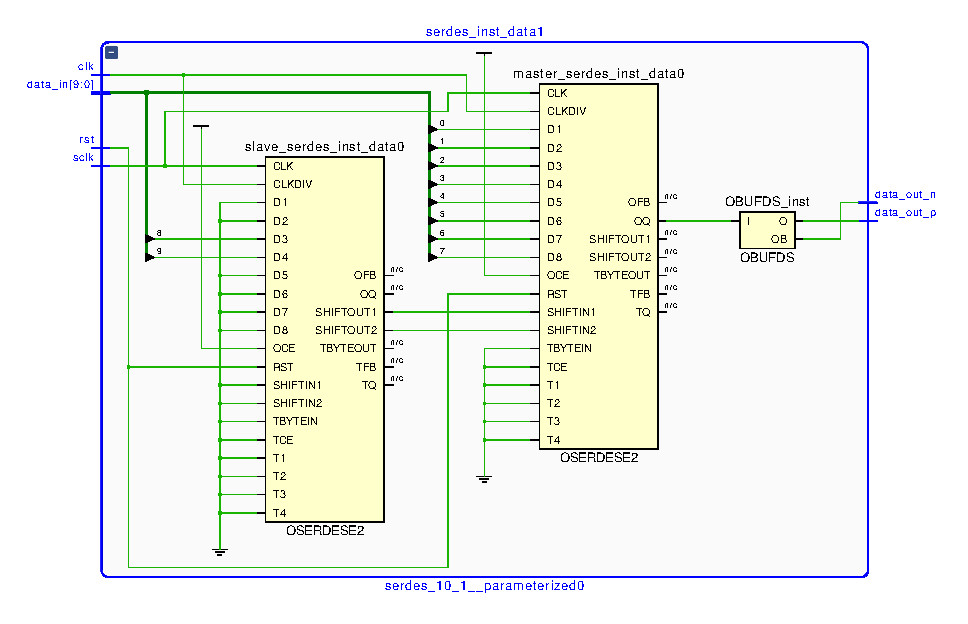
\includegraphics[scale=0.8]{serdes.pdf}
    \end{minipage}
    \item The 10-bit encoded data generated from the encoder instances are forwarded to the SerDes units. serdes\_inst instances do the task of serializing the 50-bit data over five LVDS data Lane. The fast serial clock sclk is also sent through LVDS lane using serdes\_inst instance to match the delay in clock lane with the data paths. The OSERDESE2 units have been used in the cascading configuration using the SHIFT* pins to expand the data width to 10-bit. 

% \begin{figure}[h!]
% \centering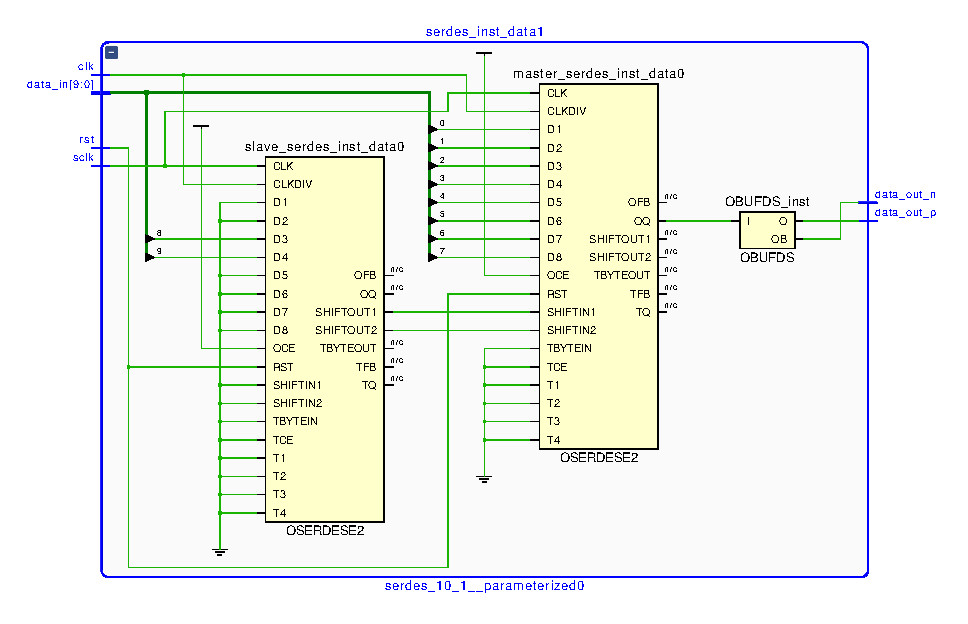
\includegraphics[scale=1]{serdes.pdf}
% \caption{OSERDESE2 configuration}
% \end{figure}
    
\end{itemize} 
\section{Receiver Gearwork}\index{Receiver Gearwork}

\begin{figure}[h!]
\centering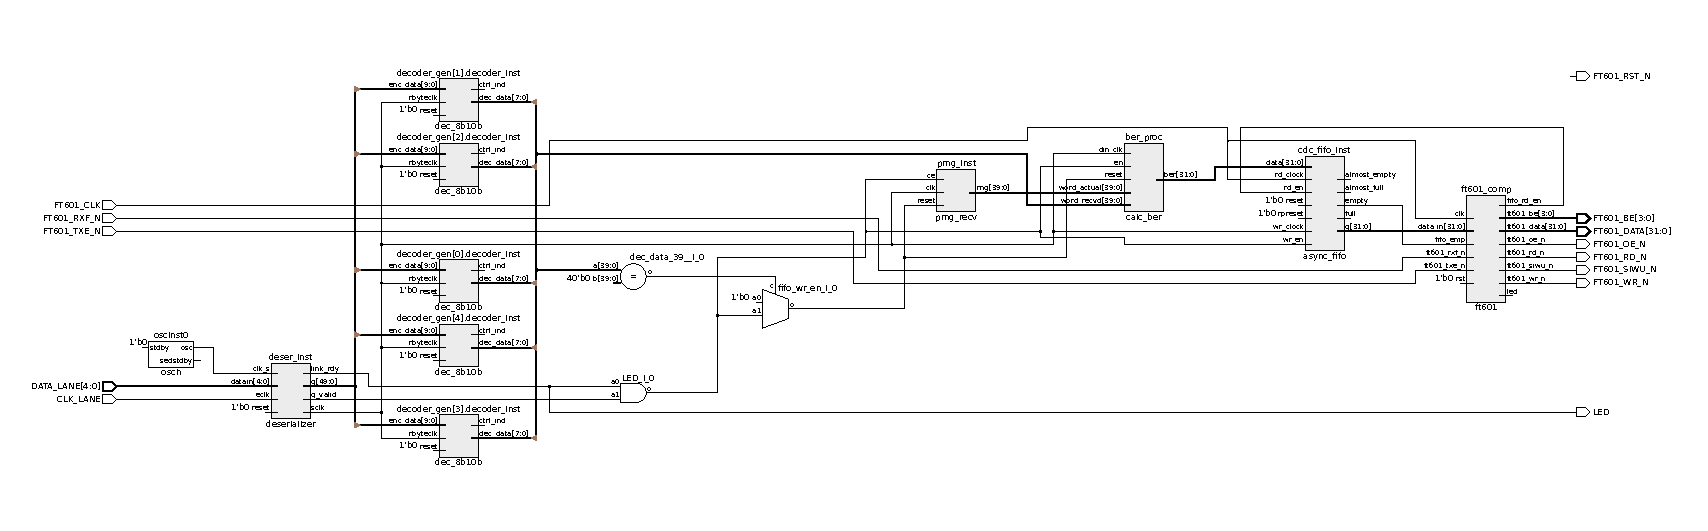
\includegraphics[scale=0.5]{MachXO2_Schematic.pdf}
\caption{MachXO2 Gearwork Schematic}
\end{figure}
The above figure describes the receiver part of model developed for BER testing.
\begin{itemize}
    \item The high speed serial links set up between the MicroZED and the plugin module follow the source synchronous system with the assumption that initially data and clock are edge-aligned. Static delays have been adjusted in the data path to achieve the same on the AXIOM Beta.
    \item The edge aligned clock is forwarded to the DLLDELC primitive which can add dynamic delay to the clock with DQSDEL delay input code from DQSDLLC primitive. DQSDLLC ensure that clock gets a 90$\degree$ phase shift, thereby making it centre aligned with the data while also adjusting for the PVT variation. \par
        \begin{minipage}{\linewidth}
        \centering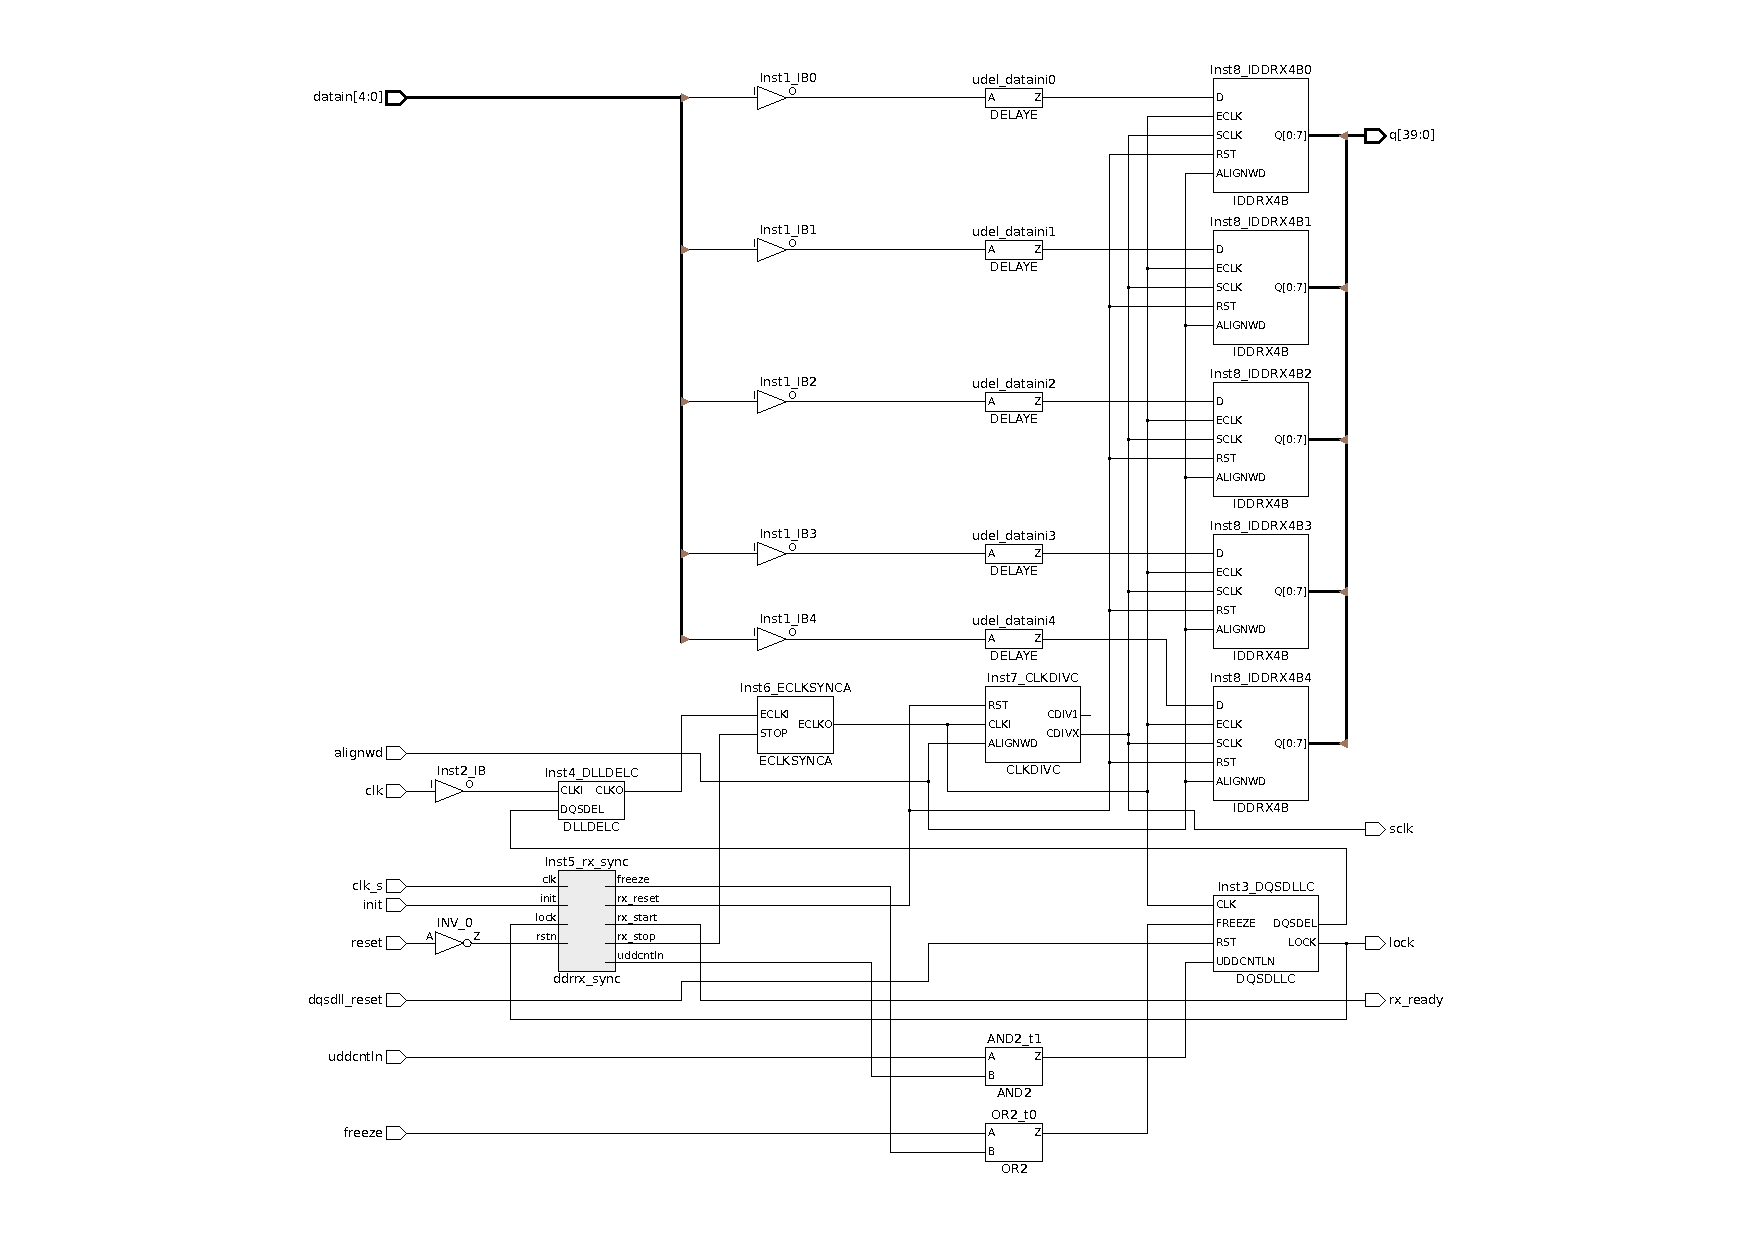
\includegraphics[scale=0.5]{DDRx4_Schematics.pdf}
        \center\caption{DDRx4 Gearing Schematic}
    \end{minipage}
    \item RX Sync is a soft IP provided by Lattice that ensures proper reset synchronization of all the IDDRX4B and CLKDIVC primitive to maintain the clock domain crossing margin between fast edge and divided word clock, and to avoid bus bit-order scrambling due to the various delay of the reset pulse. ECLKSYNCA is used to send the fast edge clock to the edges of the MachXO2 with minimum skew and also for reset synchronization of IDDRX4B \& CLKDIVC. (Refer to \textcolor{blue}{\href{https://www.latticesemi.com/view_document?document_id=39084}{ Implementing High-Speed Interfaces with MachXO2 Devices-TN1203}})
    \item As MachXO2 doesn't support 10:1 gearing, the data had to be first geared down to 8:1 with the IDDR4XB primitive, then consecutively gear down to 10:8  with a  barrel shifter.
    The IDDR4XB provides an option for bit slip with the input signal ALIGNWD, and as the lengths of all data lanes have difference of few millimeters , i.e. less than few picoseconds in terms of delay, all IDDRX4B instance need equal number of bit slip to get generate aligned words.
    \item The deserializer instance performs the link training, channel bonding, 10:8 gearing and finally outputs the five 10-bit encoded words received from each LVDS lanes at 93.75 MHz with 4/5 times valid signal.
    \item The encoded 10-bit data is sent to 8b/10b decoders where after decoding they get compared with the data generated by the PRNG instance (having the same SEED and synchronized to PRNG on Zynq using a all zeros word). The calc\_ber instance counts the number of bit errors, i.e. the number of unequal bits between the received data and the locally generated data, and updates the BER result every time after analysing $2^{30}$ 40-bit words.
    \item The 32-bit BER results are en-queued in asynchronous FIFO allowing clock domain crossing between the received data clock and the 100 MHz data input clock from the FT601 chip.
    These 32-bit BER values are then fetched by the FT601 controller instance from the FIFO and sent to the FTDI FT601 chip for conversion to USB 3.0 packets, which are then streamed to the connected PC.
    \item On the software end, we use a proprietary FTDI D3XX driver, whose documentation and APIs can be found \textcolor{blue}{\href{https://github.com/apurvanandan1997/usb_plug_mod_ber/blob/master/D3XX/README.pdf}{here}} 
\end{itemize} 
\par\noindent\rule{\textwidth}{0.4pt}
\centering ***
% \begin{figure}[h!]
% \centering\includegraphics[scale=0.5]{}
% \caption{DDR x4 gearing}
% \end{figure}

%\section{Software}\index{Software}


% %------------------------------------------------



\end{document}
